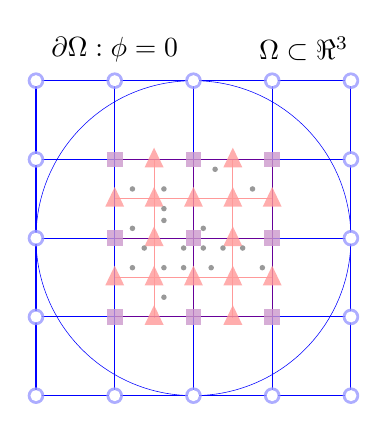
\begin{tikzpicture}[domain=-0.2:4.2,scale=1.0]
    %MG grid
    \draw[thin,color=blue,step=10mm] (0.0,0.0) grid (4,4);
    %\draw[very thin,color=gray,step=2.5mm] (0.5,-0.2) grid (3.5,1.5);
    
    %labels
    \node at (3.4,4.4) {$\Omega \subset \Re^3$};
    \node at (1,4.4) {$\partial \Omega: \phi = 0$};

    %additional grid lines MG
    %\draw[thin,color=blue] (0.5,0.0) to (0.5,4);
    %\draw[thin,color=blue] (1.5,0.0) to (1.5,4);
    %\draw[thin,color=blue] (2.5,0.0) to (2.5,4);
    %\draw[thin,color=blue] (3.5,0.0) to (3.5,4);
    
    \draw[very thin,color=blue] (2.0,2.0) circle (2);
    
    %FFT grid
    \draw[thin,color=red,step=5mm,opacity=0.4] (1.0,0.99) grid (3,3);

    %MG meshpoints
    \foreach \i in {0, 1.0, ..., 4}
    {
        \fill[blue!40,opacity=0.8] (\i,0.0) circle (3pt);
        \fill[white,opacity=1.0] (\i,0.0) circle (2pt);
    }
    \foreach \i in {0, 1.0, ..., 4}
    {
        \fill[blue!40,opacity=0.8] (\i,4.0) circle (3pt);
        \fill[white,opacity=1.0] (\i,4.0) circle (2pt);
    }
    \foreach \i in {1, ..., 3}
    {
        \fill[blue!40,opacity=0.8] (0.0,\i) circle (3pt);
        \fill[white,opacity=1.0] (0.0,\i) circle (2pt);
    }
    \foreach \i in {1, ..., 3}
    {
        \fill[blue!40,opacity=0.8] (4.0,\i) circle (3pt);
        \fill[white,opacity=1.0] (4.0,\i) circle (2pt);
    }
    
    %FFT meshpoints
    \foreach \i in {1, 1.5, ..., 3}
    {
        \fill[red!40,opacity=0.8] (\i-0.12,1.5-0.1) -- (\i,1.5+0.15) -- (\i+0.12,1.5-0.1);
    }
    \foreach \i in {1, 1.5, ..., 3}
    {
        \fill[red!40,opacity=0.8] (\i-0.12,2.5-0.1) -- (\i,2.5+0.15) -- (\i+0.12,2.5-0.1);
    }
    \foreach \j in {1.0, ..., 3.0}
    {
        \foreach \i in {1.5, ..., 2.5}
        {
            \fill[red!40,opacity=0.8] (\i-0.12,\j-0.1) -- (\i,\j+0.15) -- (\i+0.12,\j-0.1);
        }
    }
   
    %SHARED meshpoints
    \foreach \j in {1, ..., 3}
    {
        \foreach \i in {1, ..., 3}
        {
            \fill[violet!40,opacity=0.8] (\i-0.1,\j-0.1) rectangle (\i+0.1,\j+0.1);
        }
    }


    %particles
    \fill[black!40] (2.225,1.625) circle (1pt);
    \fill[black!40] (2.750,2.625) circle (1pt);
    \fill[black!40] (1.625,1.25) circle (1pt);
    
    \fill[black!40] (2.275,2.875) circle (1pt);

    \fill[black!40] (1.625,2.625) circle (1pt);
    
    \fill[black!40] (1.375,1.875) circle (1pt);

    \fill[black!40] (1.225,2.625) circle (1pt);
    \fill[black!40] (1.225,2.125) circle (1pt);
    \fill[black!40] (1.225,1.625) circle (1pt);
    
    \fill[black!40] (1.625,2.375) circle (1pt);
    \fill[black!40] (1.625,1.625) circle (1pt);
    \fill[black!40] (1.625,2.225) circle (1pt);

    \fill[black!40] (1.875,1.875) circle (1pt);
    \fill[black!40] (1.875,1.625) circle (1pt);
    
    \fill[black!40] (2.125,1.875) circle (1pt);
    \fill[black!40] (2.125,2.125) circle (1pt);

    \fill[black!40] (2.375,1.875) circle (1pt);

    \fill[black!40] (2.625,1.875) circle (1pt);
    
    \fill[black!40] (2.875,1.625) circle (1pt);

\end{tikzpicture}
